
\documentclass[a4paper, 11pt]{article}

\usepackage[czech]{babel}
\usepackage[T1]{fontenc}
\usepackage[utf8]{inputenc}
\usepackage[left=2cm, top=3cm, text={17cm, 24cm}]{geometry}
\usepackage{times}
\usepackage{graphicx}
\usepackage[unicode]{hyperref}
\usepackage[]{graphicx}
\usepackage{subcaption}
\usepackage{flafter}
\usepackage{float}
\usepackage{hyperref, xurl}
\usepackage{svg}
\usepackage{pdflscape}

\usepackage{listings}
\usepackage{xcolor}
\usepackage{color}
\usepackage{textcomp}

\hypersetup{
    pdftitle={Projektová dokumentace - Ukládání rozsáhlých dat v NoSQL databázích},
}

\makeatletter
\newcommand\footnoteref[1]{\protected@xdef\@thefnmark{\ref{#1}}\@footnotemark}
\makeatother


\lstdefinestyle{Cypher}{
    literate={á}{{\'a}}1 {é}{{\'e}}1 {ě}{{\v{e}}}1 {Č}{{\v{C}}}1 {č}{{\v{c}}}1 {ř}{{\v{r}}}1 {š}{{\v{s}}}1 {ž}{{\v{z}}}1 {í}{{\'i}}1 {ý}{{\'y}}1 {ť}{{\v{t}}}1,
    language=SQL,
    breaklines=true,        
    morekeywords={LOAD, MERGE, WITH, RETURN},
    basicstyle=\small\ttfamily,
    framexleftmargin=-55pt,
    xleftmargin=-50pt,
    framesep=10pt,
    frame=shadowbox,
    showstringspaces=false,
    backgroundcolor=\color{green!5},
    rulesepcolor=\color{cyan!5}
}

\lstdefinestyle{NoSQL}{
    literate={á}{{\'a}}1 {é}{{\'e}}1 {ě}{{\v{e}}}1 {Č}{{\v{C}}}1 {č}{{\v{c}}}1 {ř}{{\v{r}}}1 {š}{{\v{s}}}1 {ž}{{\v{z}}}1 {í}{{\'i}}1,
    language=SQL,
    basicstyle=\small\ttfamily,
    framexleftmargin=-55pt,
    xleftmargin=-50pt,
    framesep=5pt,
    frame=shadowbox,
    showstringspaces=false,
    backgroundcolor=\color{green!5},
    rulesepcolor=\color{cyan!5}
}

\lstdefinestyle{Python}{
    language=Python,
    basicstyle=\small\ttfamily,
    framexleftmargin=-55pt,
    xleftmargin=-50pt,
    framesep=5pt,
    frame=shadowbox,
    showstringspaces=false,
    backgroundcolor=\color{green!5},
    rulesepcolor=\color{cyan!5}
}
\setcounter{tocdepth}{2}

\begin{document}
	%%%%%%%%%%%%%%%%%%%%%%%%%%%%%%%% Titulní stránka %%%%%%%%%%%%%%%%%%%%%%%%%%%
	\begin{titlepage}
		\begin{center}
			
\includegraphics[width=0.77\linewidth]{FIT_logo.pdf} \\

			\vspace{\stretch{0.382}}

			\Huge{Projektová dokumentace} \\[0.3em]

			\LARGE{1.\,část\,--\,Ukládání rozsáhlých dat v NoSQL databázích} \\[0.6em]

			%\Large{Ukládání a příprava dat} \\
                \Large{Autor: David Chocholatý, Tomáš Bártů, Štěpán Bakaj \\ Kontakt: \{xchoch09, xbartu11, xbakaj00\}@stud.fit.vutbr.cz}

			\vspace{\stretch{0.618}}
		\end{center}

		{\Large
			\today
			\hfill
                Ukládání a příprava dat
			%David Chocholatý (xchoch09), Tomáš Bártů (xbartu11), Štěpán Bakaj (xbakaj00)
		}
	\end{titlepage}



	%%%%%%%%%%%%%%%%%%%%%%%%%%%%%%%% Obsah %%%%%%%%%%%%%%%%%%%%%%%%%%%%%%%%%%%%%
	\tableofcontents
	\clearpage

	%%%%%%%%%%%%%%%%%%%%%%%%%%%%%%%% Úvod %%%%%%%%%%%%%%%%%%%%%%%%%%%%%%%%%%%%%%
	\section{Úvod}

	Cílem této části projektu je analyzovat požadavky a navrhnout optimální způsob uložení rozsáhlých dat do vhodné NoSQL databáze tak, aby tato data bylo možno rychle dotazovat a aktualizovat. Celkem byly využity čtyři druhy NoSQL databází, a to: sloupcová wide-column databáze (databázový produkt Apache Cassandra), dokumentová databáze (databázový produkt MongoDB), grafová databáze (databázový produkt Neo4j) a databáze časových řad (databázový produkt InfluxDB). Veškeré použité datové sady byly převzaty z Národního katalogu otevřených dat pro statutární město Brno.

    % Společně
    \newpage
    \section{Sloupcová wide-column databáze\,---\,Apache Cassandra}

    \begin{itemize}
        \item Název datové sady: Plynulost dopravy
        \item URL: \url{https://data.gov.cz/datov%C3%A1-sada?iri=https%3A%2F%2Fdata.gov.cz%2Fzdroj%2Fdatov%C3%A9-sady%2F44992785%2F80355818055c0ea9f63750d98fd7982c}\footnote{Použitá data byla vytvořena a zveřejněna s účastí společnosti WAZE a Magistrátu města Brno.}
        \item Distribuce datové sady: CSV
    \end{itemize}

    \subsection{Rozbor charakteristik a výhod vybraného NoSQL řešení}

    \begin{enumerate}
        \item Flexibilní schéma: Struktura zaznamenávaných dat se může v průběhu času měnit. Především v databázi nejsou uvedeny veškeré údaje, které společnost WAZE poskytuje a dataset může být aktualizován o tyto hodnoty.
        \item Řídkost dat: Dataset obsahuje také sloupce, jejichž zastoupení hodnotami je velmi řídké. Pro takový typ dat se velmi hodí právě wide-column NoSQL databáze z důvodu, že jednotlivé řádky tabulky nemusejí obsahovat dvojici sloupec-hodnota pro všechny sloupce, které jsou zastoupeny v ostatních řádcích vytvořené tabulky.
        \item Snadná škálovatelnost a výkon: Wide-column databáze využívají distribuované úložiště mezi více uzly nebo servery, což umožňuje škálovatelnost a vysokou dostupnost.
    \end{enumerate}
    
    \subsection{Definice úložiště NoSQL databáze}
    Důležitými pojmy sloupcové wide-column databáze Apache Cassandra jsou páry sloupec-hodnota (anglicky \textit{column-value}), rodiny sloupců (anglicky \textit{column-families}), řádek (anglicky \textit{row}), servery a databázové uzly (anglicky \textit{servers and database nodes}):

    \begin{itemize}
        \item pár sloupec-hodnota -- hodnota dat je v daném typu databáze pro řádek ukládáná ve sloupcích v podobném smyslu, jako je tomu u relačních databází. Významným rozdílem je ovšem skutečnost, že daný sloupec je pouze reprezentován pro konkrétní řádek, přičemž řádek nemusí obsahovat všechny sloupce, které obsahují ostatní řádky stejné tabulky.
        \item rodina sloupců -- na základě struktury, že každý řádek má své vlastní sloupce,  lze související sloupce modelovat jako součást stejné rodiny sloupců.
        \item řádek -- řádek lze v tomto typu databáze chápat v podobném smyslu, jako je tomu u relačních databází.
        \item servery a databázové uzly -- wide-column databáze jsou organizovány jako distribuované úložiště, přičemž data jsou rozmístěna do více serverů nebo databázových uzlů. Jelikož wide-column úložiště využívají distribuované úložiště mezi více uzly nebo servery, je umožněna škálovatelnost a vysoká dostupnost.
    \end{itemize}

    Pro celkový kontext a pochopení Apache Cassandra je důležité si definovat další pojmy:

    \begin{itemize}
        \item Uzly -- Uzel je základní prvek v clusteru Cassandra. Každý uzel ukládá data a poskytuje služby, jako je vyhledávání dat, zápis dat a replikace dat mezi uzly.
        \item Virtuální uzly -- Virtuální uzly (vNodes) jsou koncept, který umožňuje každému uzlu zastupovat více tokenů v clusteru, což zjednodušuje operace přidávání, odebrání a vyvažování zátěže v clusteru.
        \item Servery -- Servery jsou fyzické stroje, na kterých běží instance uzlů Apache Cassandra. Každý server může hostovat jednu nebo více instancí Cassandry (uzlů).
        \item Racky -- Rack je skupina serverů.
        \item Datová centra -- Datové centrum je skupina uzlů, které jsou umístěny ve stejné fyzické lokalitě. V jeden okamžik může být cluster rozdělen do více datových center, která mohou být geograficky oddělena, což zvyšuje odolnost vůči chybám a umožňuje lokální vyhledávání dat. Každé datové centrum může obsahovat více racků.
        \item Cluster -- Cluster je sada uzlů (nodes), které pracují společně a jsou vnímány jako jednotný systém. Všechny uzly ve clusteru komunikují mezi sebou, aby zajistily konzistenci dat a vysokou dostupnost.
        
    \end{itemize}

    \begin{figure}[ht!]
        \centering
        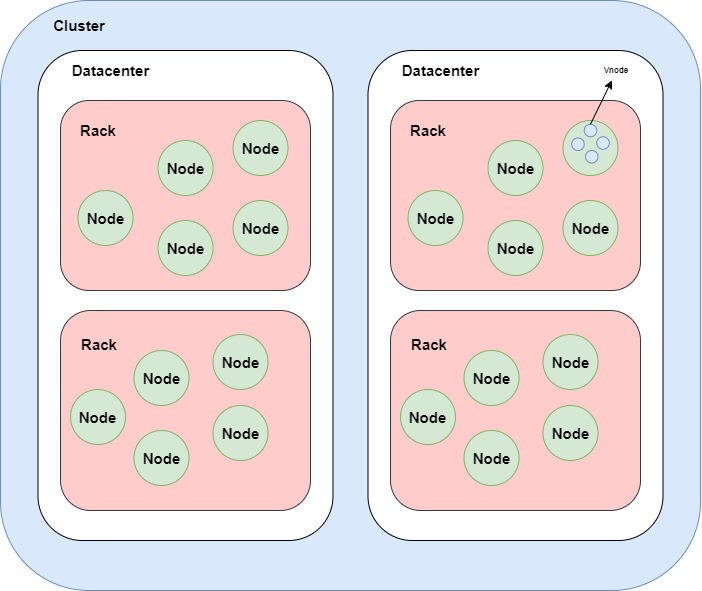
\includegraphics[width=0.75\textwidth]{img/cassandra_hierarchy.jpg}
        \caption{Hierarchie úložiště v Apache Cassandra, viz \href{https://www.baeldung.com/cassandra-cluster-datacenters-racks-nodes}{zdroj}.}
        \label{CassandraHier}
    \end{figure}
    
    \subsection{Import dat}
        Pro import dat ze zvolené datové sady do NoSQL databáze Apache Cassandra je možné použít CQL shell respektive \texttt{cqlsh} nebo Python za použití knihovny \texttt{cassandra}. V tomto projektu byl zvolen přístup za využití jazyka Python a uvedené knihovny. Postup importu dat ze zvolené datové sady vypadá následovně:

        \begin{enumerate}
            \item Příprava dat -- Stažení vybrané datové sady ve formátu CSV.
            \item Příprava prostředí -- Kontrola, zda mámě přístup k databázovému serveru Apache Cassandra a nainstalovanou knihovnu cassandra. V případě, že není nainstalovaná, lze ji nainstalovat následovně:

            \begin{lstlisting}[style=NoSQL, language=SQL, framesep=10pt]
        $ pip install cassandra-driver            
            \end{lstlisting}            

            \item Připojení k Apache Cassandra a autentizace pomocí uživatelského jména a hesla.

            \begin{lstlisting}[style=Python, language=Python, framesep=10pt]
        from cassandra.auth import PlainTextAuthProvider

        ...
        
        auth_provider = PlainTextAuthProvider(username='admin', password='admin321')
            \end{lstlisting}

            \item Vytvoření \textit{Clusteru} s kontaktním místem (anglicky \textit{ contact points}) na zadané IP adrese a portu, na kterém se otvírá spojení. Následně dochází k otevření samotného spojení.


            \begin{lstlisting}[style=Python, language=Python, framesep=10pt]
        from cassandra.cluster import Cluster

        ...
        
        cluster = Cluster(['192.168.1.8'], port=9042, auth_provider=auth_provider)
        session = cluster.connect()
            \end{lstlisting}

            \item Kontrola, zda již není již vytvořený tzv. klíčový prostor (anglicky \textit{keyspace}). Pokud ano, použije se vytvořený keyspace. V opačném případě se vytvoří nový a nastaví se jako keyspace pro otevřené spojení.

            \begin{lstlisting}[style=Python, language=Python, framesep=10pt, breaklines=true]
        # Check if the keyspace exists
        keyspace_name = args.keyspace
        keyspace_query = "SELECT * FROM system_schema.keyspaces WHERE keyspace_name = %s"
        keyspace_exists = session.execute(keyspace_query, [keyspace_name])
    
        # Create the keyspace if it doesn't exist
        if not keyspace_exists:
            create_keyspace_query = f"""
            CREATE KEYSPACE {keyspace_name}
            WITH replication = {{'class': 'SimpleStrategy', 'replication_factor': 1}};
            """
            session.execute(create_keyspace_query)
    
        session.set_keyspace(keyspace_name)
            \end{lstlisting}

            \item Vytvoření struktury tabulky, do které se budou ukládat data z vybraného datasetu. Rozmístění po serverech se provádí pomocí první části primárního klíče, a to pomocí hodnoty sloupce \texttt{level}. Dále se na jednotlivých serverech indexuje podle hodnoty \texttt{uuid}. Následně je vytvořena samotná tabulka.

            \begin{lstlisting}[style=Python, language=Python, framesep=10pt]
        create_table_query = """
        CREATE TABLE IF NOT EXISTS brno_jam (
            country text,
            level int,
            city text,
            speed_KMH int,
            length int,
            uuid int,
            end_node text,
            speed_MS int,
            blocking_Alert_Uuid text,
            road_Type text,
            delay int,
            street text,
            pub_Millis timestamp,
            PRIMARY KEY (level, uuid)
        );
        """
    
        session.execute(create_table_query)
        
            \end{lstlisting}

            \item Načtení CSV souboru a vložení dat z datasetu do vytvořené tabulky. Při načítání časových dat je vhodné převést poskytnutý časový údaj do koordinovaného světového času UTC. Následně je vytvořen příkaz pro vložení záznamu datasetu pomocí funkce \texttt{session.prepare()} a je spuštěna exekuce daného příkazu.

            \begin{lstlisting}[style=Python, language=Python, framesep=10pt, breaklines=true]
        import csv
        from datetime import datetime, timezone

        ...
    
        with open(args.file, 'r', encoding='utf-8') as file:
        reader = csv.reader(file)
        next(reader)  # Skip header row if needed
        for row in reader:
            date_string = row[16].split('+')[0].strip()
            date_object = parser.parse(date_string)
            # Convert the date object to UTC and extract the components
            date_object_utc = date_object.astimezone(timezone.utc)
            insert_query = session.prepare("INSERT INTO brno_jam (country, level, city, speed_KMH, length, uuid, end_node, speed_MS, blocking_Alert_Uuid, road_Type, delay, street, pub_Millis) VALUES (?, ?, ?, ?, ?, ?, ?, ?, ?, ?, ?, ?, ?);")
            session.execute(insert_query, (row[0], int(row[1]), row[2], int(row[3]), int(row[4]), int(row[8]), row[9], int(row[10]), row[11], row[12], int(row[13]), row[14], date_object_utc))
    
        # Close the connection to the Cassandra cluster
        cluster.shutdown()
            \end{lstlisting}
        \end{enumerate}

        Celý tento postup je zkompletován v přiloženém Python skriptu nesoucí název \texttt{cas.py} a je možné ho spustit pomocí následujícího příkazu:


        \begin{lstlisting}[style=Python, language=Python, framesep=10pt]
        $ python3 cas.py -f plynulost_dopravy.csv    
        \end{lstlisting}        

        Při spouštění se předpokládá existující soubor \texttt{plynulost\_dopravy.csv} se staženou datovou sadou. Případně je možné skript parametrizovat dle potřeb pomocí přepínačů.
    
    \subsection{Dotaz v jazyce databázového produktu}
    V následujícím seznamu bude sepsán postup jak Apache Cassandra zpracovává dotaz:

    \begin{enumerate}
        \item Lokalizace uzlů -- Po odeslání dotazu klientem je jeden z dostupných uzlů v clusteru vybrán jako \textit{koordinátor}. Vybraný koordinátor pak využívá primární klíč (případně jiný atribut, nad kterým by měl být kvůli rychlejšímu vyhledávání vytvořen index), zde atribut \texttt{level} z dotazu níže, aby určil, na kterých uzlech v clusteru jsou uložena požadovaná data.
        \item Získání dat -- Koordinátor následně pošle požadavky na uzly, které obsahují požadovaná data, kde ty uzly následně vrátí požadovaná data koordinátorovi. Dotaz může bát zpracován v jednom uzlu nebo distribuován přes více uzlů, pokud jsou data replikována na více uzlech. V našem případě pouze v jednom uzlu zásluhou nastavení Apache Cassandry, respektive nastavení replikačního faktoru na jedna.
        \item Distribuované zpracování -- Pokud je dotaz distribuován přes více uzlů, koordinátor zpracuje výsledky z různých uzlů. Zpracování výsledků může zahrnovat agregaci, řazení nebo filtrování výsledků dle kritérií dotazu tak, aby byly splněny jeho požadavky.
        \item Doručení a zpracování výsledků -- Po zpracování výsledků koordinátor doručí výsledky klientovi, který zadal dotaz. Klient poté může výsledky zpracovat podle svých potřeb, jako je zobrazení dat, uložení výsledků pro další analýzu a podobně.
    \end{enumerate}
    Samozřejmě záleží chování serveru na jeho konkrétním nastavení. 

    \subsubsection{Popis dotazu v jazyce CQL}
    V této podsekci bude popsán vybraný dotaz v jazyce CQL.

    Následující dotaz vyhledává všechny záznamy o dopravní zácpě, které jsou situovány na ulici \textit{24. dubna} dne 14. srpna roku 2022. Vybrány jsou pouze takové záznamy, které mají úroveň dopravní zácpy \texttt{5}, což značí nehybnou kolonu. Zároveň je pro spuštění dotazu nutné povolit filtrování pomocí konstrukce \texttt{ALLOOW FILTERING}.

    \begin{lstlisting}[style=NoSQL, language=SQL, framesep=10pt, morekeywords={ALLOW}]
        SELECT * FROM brno_jams.brno_jam WHERE level = 5 
            AND street = '24. dubna' 
            AND pub_Millis >= '2022-08-14 00:00:00' 
            AND pub_Millis < '2022-08-15 00:00:00' 
        ALLOW FILTERING;
    \end{lstlisting}

    Na základě exekuce dotazu bylo nalezeno ve vytvořené databázi 19 záznamů odpovídajících zadaným požadavkům.
    
    % Bárt
    \newpage
    \section{Dokumentová databáze\,---\,MongoDB}

    \begin{itemize}
        \item Název datové sady: Akce
        \item URL: \url{https://data.gov.cz/datov%C3%A1-sada?iri=https%3A%2F%2Fdata.gov.cz%2Fzdroj%2Fdatov%C3%A9-sady%2F44992785%2F65c606ff963f53849bb0101b9a4e28e3}
        \item Distribuce datové sady: GeoJSON
    \end{itemize}

    \subsection{Rozbor charakteristik a výhod vybraného NoSQL řešení}
    Vybraný dataset obsahuje geoprostorová data o různých akcích konaných v Brně z oficiálního turistického průvodce Brnem \url{www.gotobrno.cz}, který provozuje TIC BRNO, příspěvková organizace. Dataset obsahuje jak atributy popisující samotné akce (název, popis, čas konání, atd.), tak i geoprostorové souřadnice místa konání, přičemž samotný dataset je aktualizován na denní bázi. MongoDB je vhodná volba pro tento typ dat z několika důvodů a to takovýchto:

    \begin{enumerate}
        \item Flexibilní schéma -- Struktura dat o akcích se může v průběhu času měnit (například mohou být přidány nové kategorie akcí nebo další popisné informace). MongoDB umožňuje ukládat dokumenty s různou strukturou v rámci téže kolekce, což zjednodušuje práci s daty a umožňuje snadnou adaptaci na změny.
        \item  Geoprostorová podpora -- MongoDB poskytuje podporu pro práci s geoprostorovými daty, včetně možnosti vytvářet geoprostorové indexy a provádět geoprostorové dotazy. To umožňuje efektivně vyhledávat akce v závislosti na jejich geografické poloze, což je podstatné například pro nalezení akcí v konkrétní oblasti.
        \item Snadná škálovatelnost a výkon -- MongoDB je navrženo tak, aby poskytovalo vysoký výkon a škálovatelnost, což je důležité pro práci s velkými objemy dat a velkým počtem uživatelů. V případě, že počet akcí nebo počet uživatelů vyhledávajících akce v Brně vzroste, MongoDB, lze škálovat databázi přidáním dalšího serveru případně serverů.
        \item Dotazovací jazyk -- MongoDB poskytuje rozsáhlé možnosti pro dotazování a agregaci dat, což umožňuje snadno získávat informace dotazy.  Lze například snadno vytvářet dotazy, které vyhledávají akce konané v určitém časovém období nebo akce v určité oblasti.
    \end{enumerate}
    
    \subsection{Definice úložiště NoSQL databáze}
    Důležitými pojmy v MongoDB jsou databáze, kolekce a dokument. Popis jednotlivých pojmů v kontextu MongoDB jsou následující:
    \begin{itemize}
        \item databáze -- Nacházejí se na MongoDB serveru a zde jich může být několik, kde každá jedna z nich může obsahovat několik kolekcí.
        \item kolekce -- Jedna kolekce může obsahovat více dokumentů.
        \item dokument -- Jeden dokument může obsahovat více datových záznamů.
    \end{itemize}
    \newpage
    Výše vypsané pojmy jsou hierarchicky vyobrazeny na obrázku~\ref{MongoHier}:
    \begin{figure}[ht!]
        \centering
        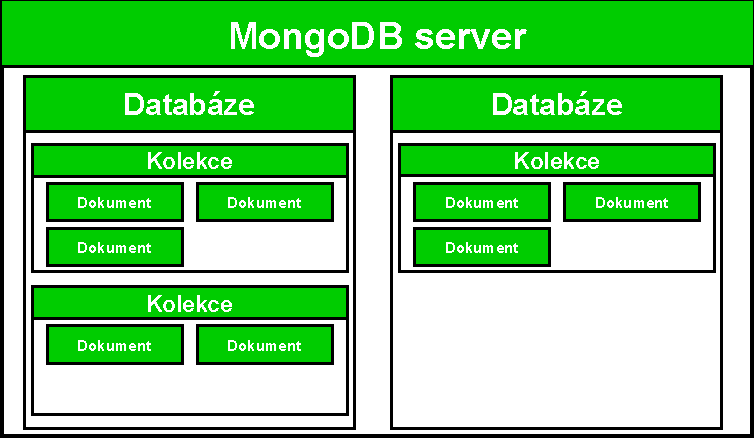
\includegraphics[width=0.85\textwidth]{img/MongoDB.pdf}
        \caption{Hierarchie úložiště v MongoDB \label{MongoHier}}
    \end{figure}
    
    Pomocí příkazu \texttt{use} společně s názvem databáze je možné vytvořit v systému novou databázi, avšak pokud již databáze s tímto názvem v systému existuje dojde pouze k přepnutí kontextu na tuto databázi. Pro vytvoření databáze s názvem \texttt{brno\_akce}. lze použít následující příkaz:
    \begin{lstlisting}[style=NoSQL, language=SQL, framesep=10pt]
        > use brno
    \end{lstlisting}
    
    V analogii s relačními SQL databázemi, jež obsahují tabulky, tak v MongoDB tabulkám odpovídají kolekce. Novou kolekci v databázi lze vytvořit příkazem \texttt{db.createCollection(\textit{name}, \textit{options})}, kde se tento příkaz používá primárně, když je potřebné specifikovat konkrétní vlastnosti nové kolekce jako například maximální počet dokumentů, který může kolekce obsahovat či po jaké době budou dokumenty označeny za neplatné a MongoDB následně odstraní dokumenty, jimž vypršela platnost. Pokud je potřeba pouze vytvořit kolekci bez konkrétní specifikace vlastností, tak MongoDB vytváří kolekci implicitně při první referenci na kolekci v odkazu. Explicitně lze vytvořit prázdnou kolekci bez specifikace vlastností následovně:
    \begin{lstlisting}[style=NoSQL, language=SQL, framesep=10pt]
        brno> db.createCollection("akce")
    \end{lstlisting}

    V případě využití geoprostorových dat a dotazování nad nimi je vhodné, aby dotazy byly co nejefektivnější. Měl by se tedy vytvořit geoprostorový index na pole obsahující geoprostorové souřadnice a to lze provést tímto příkazem:
    \begin{lstlisting}[style=NoSQL, language=SQL, framesep=10pt]
        brno> db.akce.createIndex({ location: "2dsphere" })
    \end{lstlisting}
    přičemž toto nastavení podporuje dotazy, které počítají pomocí sférické geometrie na kouli podobné Zemi a je tak vhodné pro dotazy, jenž hledají například v určitém okolí. Zároveň je vhodný pro práci s GeoJSON, jelikož podporuje různé typy geometrií jako například \texttt{Point}, \texttt{LineString} či \texttt{Polygon}.
 Oproti tomu existuje ještě nastavení \texttt{2d}, které pracuje pouze s dvou rozměrnou rovinou.
    
    V MongoDB se samotné datové záznamy označují jako dokumenty a jsou reprezentovány jako BSON dokumenty, kde BSON označuje binární JSON. Oproti JSON je BSON rozšířen o některé datové typy, které nejsou nativní v JSON jako například datum či binární data. Vložení dokumentu do kolekce je možné příkazem \texttt{db.collection.insertOne()} či \texttt{db.collection.insertMany()}, kde první z nich vloží do kolekce právě jeden dokument a druhý může do kolekce vložit jeden a více dokumentů najednou v jednom příkazu. V případě, že by se vkládalo do kolekce, jež nebyla dříve vytvořena, tak se kolekce implicitně vytvoří. Vložení dokumentu jedné \texttt{akce} do kolekce \texttt{brno\_akce}, kde kolekce může existovat, ale nemusí, je možno provést například následujícím příkazem (pro přehlednost byly atributy nahrazeny za \dots):
    \begin{lstlisting}[style=NoSQL, framesep=10pt]
        > db.akce.insertOne(
            {
                _id: 207276,
                GlobalID: '{07E6D448-AADF-496B-AA97-9AD3C301796E}',
                ID: 207276,
                ObjectId: 1,
                categories: 'Veletrhy / vzdělávací',
                date_from: '2023-11-01T00:00:00Z',
                date_to: '2023-11-01T00:00:00Z',
                ...
                location: {
                    type: 'Point',
                    coordinates: [
                        16.612533946000042,
                        49.193951619000075
                    ]
                },
                ...
                name: 'Člověk, smrtelná osobnost a&nbsp;nesmrtelné jádro',
                name_en: null,
                organizer_email: 'kancelar.rosicrucianum@gmail.com',
                parent_festivals: null,
                text: 'Srdečně zveme veřejnost na přednášku.Zkoumání cesty...',
                ...
            }
        )
    \end{lstlisting}
    \subsection{Import dat}
    Pro import dat ze zvolené datové sady do NoSQL databáze MongoDB je možné použít Mongo Shell respektive \texttt{mongosh} nebo Python za použití knihovny \texttt{pymongo}. Jelikož bude potřeba upravit počáteční data, tak je pro pohodlnější práci zvolen Python. Postup importu dat ze zvolené datové sady vypadá následovně:
    \begin{enumerate}
        \item Příprava dat -- Stažení vybrané datové sady ve formátu GeoJSON.
        \item Příprava prostředí -- Kontrola zda máme přístup k databázovému serveru MongoDB a nainstalovanou python knihovnu pymongo. V případě, že není nainstalované lze ji nainstalovat následovně:
        \begin{lstlisting}[style=NoSQL, language=SQL, framesep=10pt]
        $ pip install pymongo
        \end{lstlisting}
        \item Načtení GeoJSON souboru -- Načtení dat ze souboru a převedení jej na snadno zpracovatelná formát: 
        \begin{lstlisting}[style=Python, language=Python, framesep=10pt]
        import json
        
        with open(FILE, "r") as json_file:
        data = json.load(json_file)
        \end{lstlisting}
        \item Připojení k MongoDB -- Připojení se k MongoDB databázi a vytvoření databáze v případě, jestli již neexistuje. Následné vytvoření kolekce a v případě, že již kolekce se stejným názvem v dané databázi existuje, tak  získání pouze reference na tuto kolekci, do které se budou data importovat.
        \begin{lstlisting}[style=Python, language=Python, framesep=10pt]
        from pymongo import MongoClient
        client = MongoClient("mongodb://"+ID+":"+PASSWORD+"@"+URL+":"+str(PORT))
        db = client[DATABASE]
        collection = db[COLLECTION]
        \end{lstlisting}
        \item Příprava a import samotných dat -- Při importu dat ze zvolené distribuce GeoJSON datové sady do MongoDB kolekce je možné postupovat tak, že inicializujeme prázdný seznam \texttt{updates}, do kterého se budou postupně přidávat operace pro hromadný zápis do databáze. Pro každý prvek z datové sady získáme jeho vlastnosti --\texttt{properties} a geolokační údaje -- \texttt{geometry}. Získané geolokační údaje jsou následně vloženy přímo do \texttt{properties} pod klíčem \texttt{location}, což umožňuje vytvořit strukturovaný záznam jednotlivých akcí konaných v Brně. \texttt{ID} události je nastaveno jako \texttt{\_id} v \texttt{properties}, což zajišťuje unikátní identifikátor pro každý dokument v MongoDB. Pro každý takto připravený záznam je vytvořen objekt \texttt{UpdateOne}, který je nastaven, aby aktualizoval dokument v kolekci na základě nového \texttt{\_id}. V případě, že dokument s daným \texttt{\_id} neexistuje, je automaticky vytvořen. Toto lze nastavit pomocí parametru funkce -- \texttt{upsert=True}. Nakonec jsou všechny připravené operace uložené v poli \texttt{updates} provedeny hromadně pomocí funkce \texttt{bulk\_write}, což zajišťuje efektivní a rychlý import nebo aktualizaci dat v databázi. Výše popsaný postup je zapsán algoritmicky jako:
        \begin{lstlisting}[style=Python, language=Python, framesep=10pt]
        from pymongo import UpdateOne
        updates = []

        for feature in data["features"]:
            properties = feature["properties"]
            properties["location"] = feature["geometry"]
            _id = int(properties["ID"])
            properties["_id"] = _id
            updates.append(UpdateOne({"_id": _id}, {"$set": properties}, upsert=True))

        collection.bulk_write(updates)
        \end{lstlisting}
        \item Vytvoření geosferického indexu -- Po dokončení hromadného zápisu a aktualizace dat v databázi je podstatné zabezpečit, aby byly geolokační dotazy na databázi efektivní a rychlé a k tomuto lze využít geosférický index, který je speciálně navržený pro práci s geolokačními daty. Vytvoření geosférického indexu je realizováno funkcí \texttt{create\_index} na MongoDB kolekci, kde je jako parametr předána dvojice \texttt{("location", GEOSPHERE)}, což zajistí, aby databáze na poli \texttt{location} vytvořila geosférický index, přičemž toto pole obsahuje geolokační data akcí v Brně. Díky geosférickému indexu je možné efektivně vyhledávat záznamy na základě jejich geografické polohy. Díky tomuto indexu je možné následně provádět různé geospatiální dotazy, jako vyhledávání záznamů v určitém okruhu, vyhledávání nejbližších záznamů k danému bodu, apod.
        \begin{lstlisting}[style=Python, language=Python, framesep=10pt]
        from pymongo import GEOSPHERE

        collection.create_index([("location", GEOSPHERE)])
        \end{lstlisting}
        
    \end{enumerate}
    Celý tento postup je zkompletován v přiloženém Python skriptu nesoucí název \texttt{mongodb.py} a je možné ho spustit pomocí 
    následujícího příkazu příkazu:
    \begin{lstlisting}[style=Python, language=Python, framesep=10pt]
        $ python3 mongodb.py -f akce.geojson -d brno -c akce -a store
    \end{lstlisting}
    Při spouštění se předpokládá existující soubor \texttt{akce.geojson} se staženou datovou sadou. Případně je možné skript parametrizovat dle potřeb pomocí přepínačů.
    
    \subsection{Dotaz v jazyce databázového produktu}
    Pro správné pochopení, jak MongoDB zpracovává dotaz, je možné postup rozdělit do několika klíčových kroků, kde jednotlivé kroky postupu jsou popsány níže
    \begin{enumerate}
        \item Distribuované zpracování -- V distribuovaném prostředí, jako je může být dotaz rozeslán na více uzlů pro paralelní zpracování.
        \item Indexace a vyhledávání --  Indexy umožňuje efektivní procházení stromové struktury a tím i vyhledávání dokumentů. Pro dotaz zmíněný níže se při vyhledávání použije předem vytvořený geosférický index na poli \texttt{location} pro rychlé vyhledávání dokumentů. MongoDB používá pro vyhledávání B-stromy pro většinu indexů, ale pro geosférické indexy, které jsou použity pro vyhledávání prostorových dat, používá R-stromy\footnote{\url{https://www.linkedin.com/pulse/geo-spatial-data-queries-mongodb-how-works-r-tree-indexing-joshi\#:\~:text=The\%20R,designed\%20for\%20indexing\%20multi}}.
        \item Filtrace -- Po nalezení záznamů v indexu se provede filtrace pro zajištění, že výsledky odpovídají zadaným požadavkům dotazu (v tomto případě vzdálenost do 500 metrů od zadaného bodu), přičemž v případě distribuovaného prostředí můžou být operace, jako je řazení a agregace, na různých uzlech prováděny paralelně, což zvyšuje rychlost zpracování.
        \item Agregace výsledků -- Výsledky z jednotlivých uzlů se zkompletují a jsou vráceny jako výsledek dotazu.
        \item Konzumace výsledků -- Klient může výsledek zpracovat dle svých potřeb. Například může iterovat přes vrácený seznam dokumentů a dále jej upravovat nebo jej může jednoduše zobrazit.
    \end{enumerate}
    \newpage
    V Pythonu pomocí knihovny \texttt{pymongo} lze provádět i dotazování a to i na geolokační data. Níže je uveden příklad dotazu, který hledá události v blízkosti zadaných geografických souřadnic \texttt{longitude}, \texttt{latitude} (jedná se o geografické souřadnice Fakulty informačních technologií Vysokého učení technického v Brně) v~maximální vzdálenosti 500 metrů.
    
    \begin{lstlisting}[style=Python, language=Python, framesep=10pt]
        latitude = 49.22655516496612
        longitude = 16.595914968837057
    
        nearby_events = collection.find({
            "location": {
                "$near": {
                    "$geometry": {
                        "type": "Point",
                        "coordinates": [longitude, latitude]
                    },
                    "$maxDistance": 500
                }
            }
        })
    \end{lstlisting}
    Samozřejmě je možné se dotazovat přímo v jazyce databázového produktu, přičemž shodný dotaz zobrazený výše lze zadat do příkazová řádky MongoDB, respektive \texttt{mongosh} za předpokladu přepnutého kontextu na databázi \texttt{brno} následovně: 
    \begin{lstlisting}[style=NoSQL, language=SQL, framesep=10pt]
        brno> db.akce.find({
            "location": { 
                "$near": { 
                    "$geometry": { 
                        "type": "Point", 
                        "coordinates": [16.595914968837057, 49.22655516496612] 
                    }, 
                    "$maxDistance": 500 
                } 
            } 
        })
    \end{lstlisting}
    Rovněž jako při importování datové sady do MongoDB, tak i pro ukázku příkladu dotazu nad daty je možné použít přiložený Python skript pomocí následujícího příkazu:
    \begin{lstlisting}[style=Python, language=Python, framesep=10pt]
        $ python3 mongodb.py -f akce.geojson -d brno -c akce -a load
    \end{lstlisting}
    \newpage
    Pro názornou ukázku jak je možné pracovat s vybranou datovou sadou a databázovým produktem MongoDB je výstup dotazu zanesen do mapy za pomoci Python knihovny \texttt{folium}. Následně je samotná mapa uložena do souboru \texttt{map.html}. Vizualizovaných obsah tohoto souboru lze vidět na obrázku~\ref{MongoDB_map}.
    \begin{figure}[ht!]
        \centering
        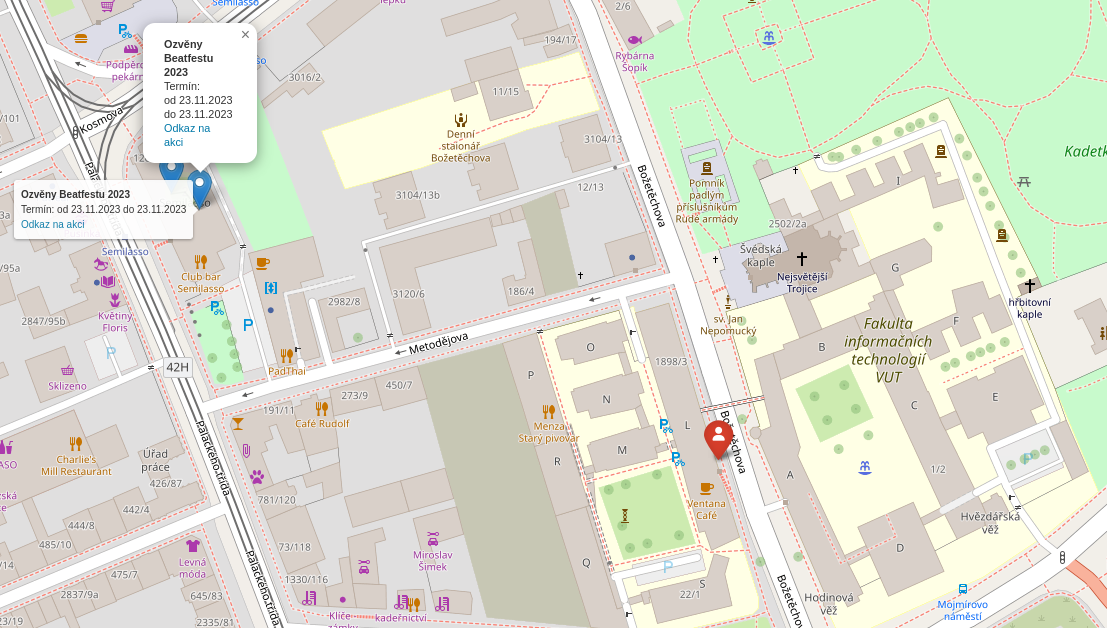
\includegraphics[width=1\textwidth]{img/mapa.png}
        \caption{Názorný příklad, jak je možné zpracovávat výsledky dotazů v MongoDB nad geolokačními daty \label{MongoDB_map}}
    \end{figure}
    % David
    \newpage
    \section{Grafová databáze\,---\,Neo4j}

    \begin{itemize}
        \item Název datové sady: Dopravní nehody
        \item URL: \url{https://data.gov.cz/datov%C3%A1-sada?iri=https%3A%2F%2Fdata.gov.cz%2Fzdroj%2Fdatov%C3%A9-sady%2F44992785%2Ff7604237598371dd478232df3ad93ce9}
        \item Distribuce datové sady: CSV
    \end{itemize}

    \subsection{Rozbor charakteristik a výhod vybraného NoSQL řešení}
    V grafové databázi jsou data uložena ve formě grafu, a to pomocí uzlů (anglicky \textit{nodes}), relací (anglicky \textit{relations}) a jejich vlastností (anglicky \textit{properties}). Hlavním cílem pro uložení dat uvedeným přístupem nejčastěji bývá potřeba zachycení vztahů (relací) mezi jednotlivými entitami (uzly) a to velmi často v rozsáhlých hierarchických datech.

    \begin{enumerate}
        \item Fixní schéma: Na základě ukládaných dat lze předpokládat, že by se struktura dat na základě zaznamenávaných informací neměla výrazně často v budoucnu měnit.

        \item Struktura dat: Pro typ grafové databáze jsou vhodné takové datové sady, ve kterých se pro jednotlivé sloupce velmi často opakují hodnoty, které obsahují. Ideálně pak, pokud sloupec může obsahovat hodnoty pouze z nějaké omezené množiny povolených hodnot. Dále je vhodné také uložit v tomto typu NoSQL databáze takovou datovou sadu, v níž dochází velmi často k duplikaci hodnot v jednotlivých řádcích.

        Tomuto popisu nejlépe odpovídá zvolená datová sada s názvem „Dopravní nehody“. V této datové sadě nejen, že v jednotlivých sloupcích dochází k duplikacím hodnot z důvodu omezeného počtu povolených validních hodnot, ovšem řádky reprezentují jednotlivé účastníky nehody, co se týče osob. To tedy znamená, že hodnoty jednoho řádku databáze odpovídají jedné osobě, které se účastnila nehody, a to ať už se jedná o řidiče nebo spolujezdce. Nutně vyplývá, že pokud se jedné dopravní nehody účastní větší počet osob, informace vztahující se pouze k záznamu nehody jsou duplikovány pro každou zúčastněnou osobu a významná část datové sady obsahuje pouze duplikovaná data.

        \item Zachycení relací: Dalším důvodem použití grafové databáze je potřeba zachycení vztahů mezi jednotlivými entitami. V našem konkrétním případě se nejčastěji požaduje zkoumat u dopravních nehod jejich vzájemná propojenost, příčiny a aspekty, které vedly ke vzniku nehody, podmínky při nehodě a další tak, aby bylo možné provést opatření, která budou v budoucnu snižovat počet dopravních nehod.

        \item Zdroj dat, frekvence a perioda aktualizace: Záznamy pocházejí z dat Policie České republiky, přičemž bezpochyby se jedná o důvěryhodný zdroj. Data jsou aktualizována jednou ročně. Nejedná se tedy o jejich příliš časté aktualizování, což může být chápáno jako výhoda pro zvolení grafové databáze.

        \item Škálovatelnost a výkon: U grafové databáze Neo4j jsou data ukládána ve formě grafu (anglicky \textit{native graph storage}). Benefitem nativního úložiště grafů je především škálovatelnost a výkon. Jedná se o optimální uložení na základě budoucích úkonů požadovaných s daným typem datové sady. V konkrétním typu NoSQL databáze se k dotazování přistupuje jako k procházení grafu na základě nativního zpracování grafu (anglicky \textit{native graph processing}) s využitím bezindexového sousedství (anglicky \textit{index-free adjacency}). Tím lze efektivně získávat požadované informace. Za účelem dosažení větší efektivity je navíc dále možné v databázovém produktu Neo4j vytvářet indexy, které napomáhají procesu nacházení specifických uzlů v grafu (pozn.: převzato ve formě parafráze\footnote{\textit{Graph Databases --  Ian Robinson, Jim Webber a Emil Eifrem, 2. vydání,} \url{https://neo4j.com/graph-databases-book/}}).

    \end{enumerate}

    
        
    \subsection{Definice úložiště NoSQL databáze}
    Důležitými pojmy grafové databáze Neo4j jsou uzly, relace a vlastnosti.

    \begin{itemize}
        \item uzel (anglicky \textit{node}) -- reprezentuje entitu vzhledem k relacím
        \item relace (anglicky \textit{relation}) -- zachycuje vztah mezi dvěma entitami reprezentovanými uzly
        \item vlastnost (anglicky \textit{property}) -- popisuje blíže uzel nebo relaci pomocí páru klíč-hodnota
    \end{itemize}

    Pro definici úložiště a následně pro vytváření dotazů byl použit dotazovací jazyk pro grafové databáze -- \textit{Cypher}. Následně jsou popsány jednotlivé části definici úložiště, přičemž jednotlivé konstrukce lze nalézt v přiloženém souboru \textit{data.cypher}.

    \begin{enumerate}
        \item Načtení datové sady z csv souboru.
        
        Při načítání dat se používá soubor z oficiálních webových stránek s datasety města Brno. Od záznamu datasetu s číslem 66 975 se struktura dat liší, jelikož se jedná pouze o nehody, ve kterých figurují chodci. Jelikož taková struktura dat není vhodná, nebudou tyto záznamy dále uvažovány (bylo by účelné rozdělit taková data do dvou datových sad). Pro demonstrační účely byla načtená datová sada omezena na 2000 záznamů.
        
    \begin{lstlisting}[style=Cypher]
        LOAD CSV WITH HEADERS FROM "https://data.brno.cz/datasets/mestobrno::dopravn%C3%AD-nehody-traffic-accidents.csv" AS row WITH row LIMIT 2000
    \end{lstlisting}

        \item Vytváření uzlů a jejich vlastností.

        Jako popisky uzlů byly zvoleny důležité entity datové sady, a to: Nehoda, MC (městská část), ZSJ (základní sídelní jednotka), Místo (přesné místo nehody), Vozidlo, Osoba, Hlavní příčina, Příčina, Povětrnostní podmínky, Rozhled, Stav vozovky, Viditelnost a Zavinění. Důvody, proč právě uvedené entity byly zvoleny jako uzly, jsou takové, že se jedná o potenciálně důležité aspekty dopravní nehody, které s velkou pravděpodobností budou při práci s databází dotazovány. Zbylé entity jsou uloženy ve formě vlastností jednotlivých uzlů nebo relací.
    \begin{lstlisting}[style=Cypher]
        MERGE (nehoda:Nehoda {id: toInteger(row.id)}) ON CREATE SET nehoda.usmrceno_os = row.usmrceno_os, nehoda.tezce_raneno_os = row.tezce_raneno_os, nehoda.lehce_raneno_os = row.lehce_raneno_os, nehoda.nasledky = row.nasledky, nehoda.hmotna_skoda = row.hmotna_skoda
        MERGE (mc:MC {mc_val: row.MC})
        MERGE (zsj:ZSJ {zsj_val: row.ZSJ})
        MERGE (misto:Misto {d: toFloat(row.d), e: toFloat(row.e)}) ON CREATE SET misto.x = toFloat(row.x), misto.y = toFloat(row.y), misto.misto_nehody = row.misto_nehody, misto.druh_komunikace = row.druh_komun, misto.situovani = row.situovani
        MERGE (vozidlo:Vozidlo {id: toInteger(row.id + row.id_vozidla), druh_vozidla: row.druh_vozidla})
        MERGE (osoba:Osoba {id: toInteger(row.OBJECTID)}) ON CREATE SET osoba.vek_skupina = row.vek_skupina IS NOT NULL, osoba.pohlavi = row.pohlavi IS NOT NULL, osoba.stav = row.stav_ridic IS NOT NULL, osoba.smrt = row.smrt, osoba.smrt_dny = row.smrt_dny, osoba.lehke_zraneni = row.lz, osoba.tezke_zraneni = row.tz, osoba.nasledek_text = row.nasledek IS NOT NULL, osoba.alkohol = row.alkohol, osoba.alkohol_vinik = row.alkohol_vinik
        MERGE (hlavni_pricina:HlavniPricina {hlavni_pricina_val: row.hlavni_pricina})
        MERGE (pricina:Pricina {pricina_val: row.pricina})
        MERGE (povetrnostni_podm:PovetrnostniPodm {povetrnostni_podm_val: row.povetrnostni_podm})
        MERGE (rozhled:Rozhled {rozhled_val: row.rozhled})
        MERGE (stav_vozovky:StavVozovky {stav_vozovky_val: row.stav_vozovky})
        MERGE (viditelnost:Viditelnost {viditelnost_val: row.viditelnost})
        MERGE (zavineni:Zavineni {zavineni_val: row.zavineni})
    \end{lstlisting}

    \item Vytváření vztahů a jejich vlastností.

    Při vytváření uzlů byly zachyceny vztahy mezi jednotlivými entitami, které jsou reprezentovány jako uzly, a to dle následujících bodů:

    \begin{itemize}
        \item Nehoda se stala \textit{lokací v} nějakém místě.
        \item Dané místo \textit{spadá do} základní sídelní jednotky.
        \item Základní sídelní jednotka \textit{náleží} městské části.
        \item Nehody \textit{se zúčastnilo} vozidlo.
        \item Osoba \textit{patřila k} nějakému vozidlu.
        \item Nehoda \textit{vznikla z} nějaké příčiny.
        \item Nehoda \textit{se stala za} určitých povětrnostních podmínek.
        \item Situaci nehody \textit{odpovídal} rozhled.
        \item Nehoda se stala \textit{při stavu} vozovky.
        \item Nehoda se stala \textit{při} určité viditelnosti.
        \item Nehoda se stala \textit{z důvodu} zavinění, ať již osoby či dalších okolností.
    \end{itemize}

    Některé relace obsahují ještě také vlastnosti. Nejprve relace mezi nehodou a místem obsahuje časové údaje týkající se doby vzniku nehody. Dále relace mezi osobou a vozidlem zachycuje pomocí vlasností vztah k vozidlu (nejobecněji řidič nebo spolujezdec) a informaci, zda byla osoba při vzniku nehody připoutána bezpečnostními pásy.

    \begin{lstlisting}[style=Cypher]
        MERGE (nehoda)-[rel_lokaci_v:LOKACI_V {datum: row.datum, den: row.den, mesic_t: row.mesic_t, rok: row.rok, mesic: row.mesic, doba: row.doba, cas: row.cas, hodina: row.hodina, den_v_tydnu: row.den_v_tydnu}]->(misto)
        MERGE (misto)-[rel_spada_do:SPADA_DO]->(zsj)
        MERGE (zsj)-[rel_nalezi:NALEZI]->(mc)
        MERGE (nehoda)-[rel_se_zucastnilo:SE_ZUCASTNILO {srazka: row.srazka}]->(vozidlo)
        MERGE (osoba)-[rel_patrila_k:PATRILA_K {vztah_k_vozidlu: row.osoba IS NOT NULL, ozn_osoba: row.ozn_osoba IS NOT NULL}]->(vozidlo)
        MERGE (nehoda)-[rel_vznikla_z:VZNIKLA_Z]->(pricina)
        MERGE (pricina)-[rel_zahrnuta:ZAHRNUTA]->(hlavni_pricina)
        MERGE (nehoda)-[rel_se_stala_za:SE_STALA_ZA]->(povetrnostni_podm)
        MERGE (nehoda)-[rel_odpovidal:ODPOVIDAL]->(rozhled)
        MERGE (nehoda)-[rel_pri_stavu:PRI_STAVU]->(stav_vozovky)
        MERGE (nehoda)-[rel_pri:PRI]->(viditelnost)
        MERGE (nehoda)-[rel_z_duvodu:Z_DUVODU]->(zavineni);
    \end{lstlisting}

    \item Vytváření indexů.

    Při definici byly vytvořeny indexy pro zefektivnění vyhledávání pro některé vybrané vlastnosti u nichž se předpokládá, že budou často vyhledávány. Konkrétně se jedná o identifikaci nehody, název městské části, název základní sídelní jednotky, druh vozidla (především pro vyhledávání nehod s účastí dopravních prostředků městské hromadné dopravy, a to tramvaje a autobusy), zavinění nehody vlivem alkoholu a příčina nehody.

    \begin{lstlisting}[style=Cypher]
        // Vytvareni RANGE indexu pro identifikator nehody.
        CREATE INDEX nehoda_index IF NOT EXISTS FOR (nehoda:Nehoda) on nehoda.id;
        // Vytvareni TEXT indexu.
        CREATE TEXT INDEX mc_index IF NOT EXISTS FOR (mc:MC) ON mc.mc_val;
        CREATE TEXT INDEX zsj_index IF NOT EXISTS FOR (zsj:ZSJ) ON zsj.zsj_val;
        CREATE TEXT INDEX vozidlo_index IF NOT EXISTS FOR (vozidlo:Vozidlo) ON vozidlo.druh_vozidla;
        CREATE TEXT INDEX osoba_alkohol_index IF NOT EXISTS FOR (osoba:Osoba) ON osoba.alkohol_vinik;
        CREATE TEXT INDEX pricina_index IF NOT EXISTS FOR (pricina:Pricina) ON pricina.pricina;
    \end{lstlisting}

    \end{enumerate}

    Vizualizace definice dat ve formě grafu je vyobrazena na obrázku \ref{data_graph}.

    \begin{figure}[ht!]
        \centering                
        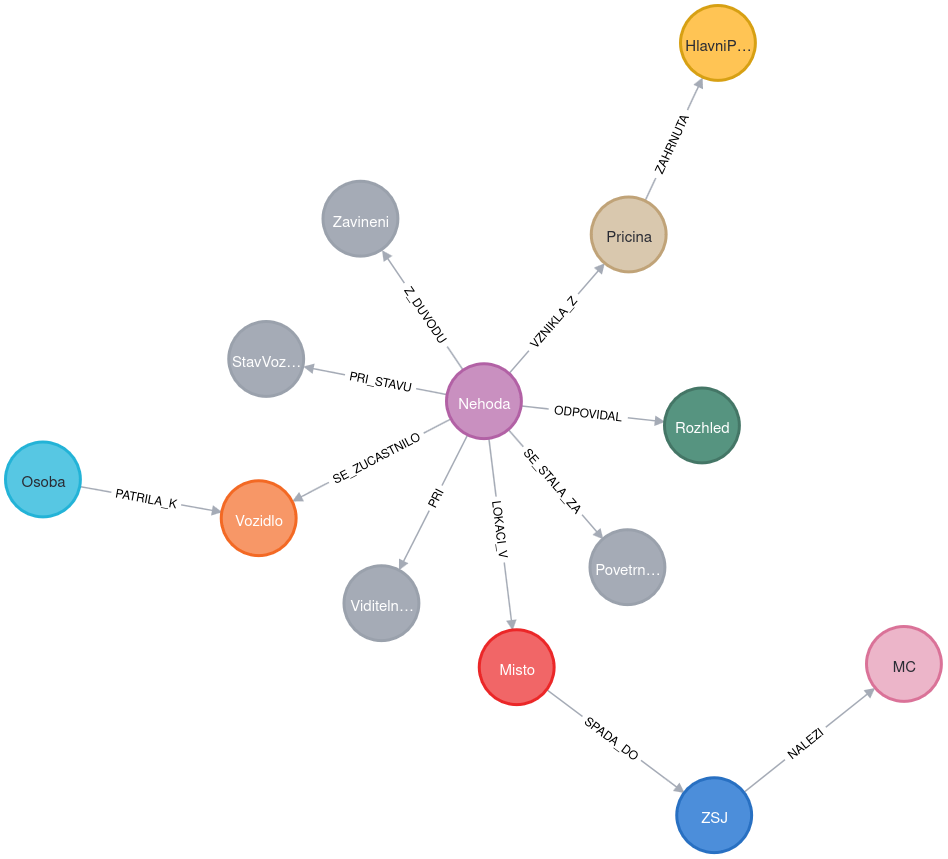
\includegraphics[width=0.9\textwidth]{img/graph_data.png}
        \caption{Graf definice dat.\label{data_graph}}
    \end{figure}

    \subsection{Import dat}
    V předchozí sekci již byla popsána sémantika jednotlivých částí kódu pro definici úložiště. V této sekci budou stejné části rozebrány z algoritmického pohledu včetně práce s aplikací Neo4j Browser. Následně bude popsáno aktualizování hodnot vytvořeného úložiště.

    \subsubsection{Popis importu dat}
    
    V této podsekci bude popsána příprava prostředí pro další práci s grafovou  databází Neo4j. Následně bude algoritmicky popsán postup importu dat do databáze.

    \begin{enumerate}        
        \item Příprava prostředí.

        Pokud je databázový produkt Neo4j nainstalován na konkrétním zařízení, je možné pracovat dále s databází s využitím uživatelsky přívětivé webové aplikace, pokud je nainstalována, \textit{Neo4j Browser}.

        Po spuštění aplikace je nejprve nutné provést připojení k serveru. To lze pomocí zadání přihlašovacích údajů a příkazu:

        \begin{lstlisting}[style=Python, language=Python, framesep=10pt]
        $ :server connect
        \end{lstlisting}

        Nejjednodušší možností definování databáze v aplikaci Neo4j Browser je vložení obsahu souboru \textit{data.cypher} do interaktivního příkazového řádku.

        Jelikož v komunitní verzi produktu Neo4j není povolené vytváření více databází, budeme pracovat s již vytvořenou výchozí databází s názvem \textit{neo4j}.
        
        \item Načtení datové sady z csv souboru.
        Jako distribuce datové sady byl vybrán csv soubor. Jeho načtení probíhá s využitím konstrukce \texttt{LOAD CSV}, která umožňuje načítání csv souboru také z URI. Následně se data získávají přímo z webových stránek s datasety města Brno pro získání aktuálních dat. Zároveň s touto konstrukcí je omezen počet řádků konstrukcí \texttt{WITH row LIMIT 2000}.
        
        \item Vytváření uzlů a jejich vlastností.
        Vytváření uzlů je prováděno pomocí klíčového slova \texttt{MERGE}. Tím je zajištěno, že pokud v databázi již existuje uzel s daným popiskem, jeho hodnoty jsou aktualizovány a nedochází k jeho duplikaci. V opačném případě je vytvořen nový uzel s příslušnými vlastnostmi. Konkrétně pro jednotlivé uzly byly zvoleny popisky tak, aby se jednalo o unikátní hodnoty v rámci databáze pro danou entitu.
        
        \item Vytváření vztahů a jejich vlastností.
        Vytváření vztahů je opět prováděno pomocí klíčového slova \texttt{MERGE}, a to ze stejných důvodů jako v předchozím případě.
        
        \item Vytváření indexů.
        Vytváření indexů je prováděno pomocí klíčového slova \texttt{CREATE INDEX}, případně \texttt{CREATE TEXT INDEX}. Vyplývá, že v databázi jsou použity dva druhy indexů, a to tzv. \texttt{RANGE} a \texttt{TEXT} indexy. Při vytváření indexů je nutné klást důraz na to, že indexy jsou idempotentní. Pro zabránění znovuvytváření již vytvořených indexů je zapotřebí při konstrukci dodat klíčového slovo \texttt{IF NOT EXISTS}. Tím je docíleno, že již existující indexy nejsou duplikovány.
    \end{enumerate}

    \subsubsection{Vkládání nových a aktualizace stávajících dat v databázi}
    Jak již bylo uvedeno, při konstrukci uzlů a relací pomocí klíčového slova \texttt{MERGE} je zabráněno duplikaci již existujících uzlů. To znamená, že například pokud je v databázi již uložena nehoda s daným identifikátorem, který je zvolen jako popisek daného uzlu, budou pouze aktualizovány hodnoty vlastností stávajícího uzlu. V opačném případě bude vložen nový uzel (\textit{upsert}). To stejné platí i při pokusu o znovuvytvoření již existující relace.

    Rovněž při konstrukci indexů bylo zabráněno jejich duplikaci pomocí klauzule \texttt{IF NOT EXISTS}.

    Pro demonstraci funkčnosti popsaných postupů je možné se pokusit načíst data znovu pomocí spuštění stejných příkazů obsažených ve skriptu. Případně je možné zkusit spustit následující část kódu (z přiloženého souboru \textit{upsert.cypher}), ve které je snaha o vytvoření již existujícího uzlu, relace a indexu.
    
    \begin{lstlisting}[style=Cypher]        
        MERGE (mc:MC {mc_val: 'Brno-střed'});
        MERGE (zsj:ZSJ {zsj_val: 'Zelný trh'})-[rel_nalezi:NALEZI]->(mc:MC {mc_val: 'Brno-střed'});
        CREATE INDEX nehoda_index IF NOT EXISTS FOR (nehoda:Nehoda) on nehoda.id;
    \end{lstlisting}

    To, že nebyly provedeny žádné změny, je potvrzeno pomocí výpisu: \textit{"(no changes, no records)"}. V případě vkládání nových dat by za použití stejných konstrukcí byl vložen nový uzel/relace/index.

    \subsection{Dotaz v jazyce databázového produktu}
    Neo4j obsahuje kompilátor, který překládá dotaz na exekuční plán, který popisuje množinu datových operací uspořádaných tak, že data jsou získávána z grafu a zpracovávána postupně pro každou operaci, dokud není pro uživatele vygenerován výsledek\footnote{\url{https://neo4j.com/blog/understanding-neo4j-cypher-queries-evaluated/}}.

    Když je Cypher dotaz spuštěn nad grafem, provedou se následující kroky:

    \begin{enumerate}
        \item Pokud dotaz ještě není v mezipaměti plánu provádění, je dotaz zkompilován do plánu provádění v Neo4j DBMS.
        \item Prováděcí plán se spustí v Neo4j DBMS k načtení dat. Mezipaměť stránek se používá k uložení dat v paměti. Paměť haldy se také používá k uložení dat meziprovozu používaných pro agregaci, řazení a vytváření cest.
        \item Neo4j DBMS vrací výsledky klientovi\footnote{\url{https://neo4j.com/graphacademy/training-cqt-40/01-cqt-40-how-queries-work-in-neo4j/}}.
    \end{enumerate}

    \subsubsection{Vysokoúrovňový popis kroků zpracování dotazu}
    Cypher dotaz začíná jako deklarativní dotaz reprezentovaný jako řetězec, popisující vzor grafu, který se má v databázi porovnat. Po analýze prochází řetězec dotazu optimalizátorem dotazů (také známým jako \textit{plánovač}), který vytvoří imperativní plán, známý jako logický plán, k určení nejúčinnějšího způsobu provedení dotazu vzhledem k aktuálnímu stavu databáze. Relevantní informace o aktuálním stavu databáze zahrnují dostupné indexy a omezení a také různé statistiky, které databáze udržuje. Plánovač Cypher používá tyto informace k určení, které vzory přístupu vytvoří nejlepší plán provedení\footnote{\label{note1}\url{https://neo4j.com/graphacademy/training-cqt-40/01-cqt-40-how-queries-work-in-neo4j/}}. Popsaný konstrukt je vyobrazen na obrázku \ref{high_level_neo4j}, který je převzat z oficiálních stránek Neo4j\footnoteref{note1}.

    \begin{figure}[ht!]
        \centering        
        \includesvg[scale=0.9]{img/high_level.svg}
        \caption{Vyobrazení zpracování Cypher dotazu v Neo4j na vyšší úrovni logiky\label{high_level_neo4j}.}
    \end{figure}
    
    V konečné fázi se tento logický plán změní na spustitelný fyzický plán, který ve skutečnosti spustí dotaz proti databázi\footnoteref{note1}.
    
    \subsubsection{Nízkoúrovňový popis kroků zpracování dotazu}
    Uvedený vysokoúrovňový popis zpracování Cypher dotazu v Neo4j je možné ještě dále rozebrat na jednotlivé části řetězce zpracování, a to následovně:

    \begin{enumerate}
        \item Dotaz je tokenizován a poté analyzován do abstraktního syntaxového stromu (AST).
        \item Sémantická kontrola se provádí na AST, aby se ujistil, že typy proměnných a rozsahy jsou platné. V opačném případě je klientovi vrácena chyba.
        \item AST je optimalizována tak, že určitá syntaxe je normalizována.
        \item Normalizované AST se používá k vytvoření grafu dotazu, který se používá k vytvoření plánu logického provádění. Plánovač pak využije své znalosti metadat grafu k vytvoření plánu fyzického provádění, což je optimalizovaná verze plánu logického provádění.
        \item Plán fyzického provádění běží v příslušném běhovém prostředí, které je založeno na operacích v plánu provádění. Některé operace nemohou běžet paralelně, takže to ovlivní, které běhové prostředí se použije k provedení dotazu. Nakonec jsou navráceny výsledky klientovi\footnote{\label{note2}\url{https://neo4j.com/graphacademy/training-cqt-40/01-cqt-40-how-queries-work-in-neo4j/}}.
    \end{enumerate}

    Popsaný konstrukt je vyobrazen na obrázku \ref{high_level_neo4j}, který je převzat z oficiálních stránek Neo4j\footnoteref{note2}.
    
    \begin{figure}[H]
        \centering        
        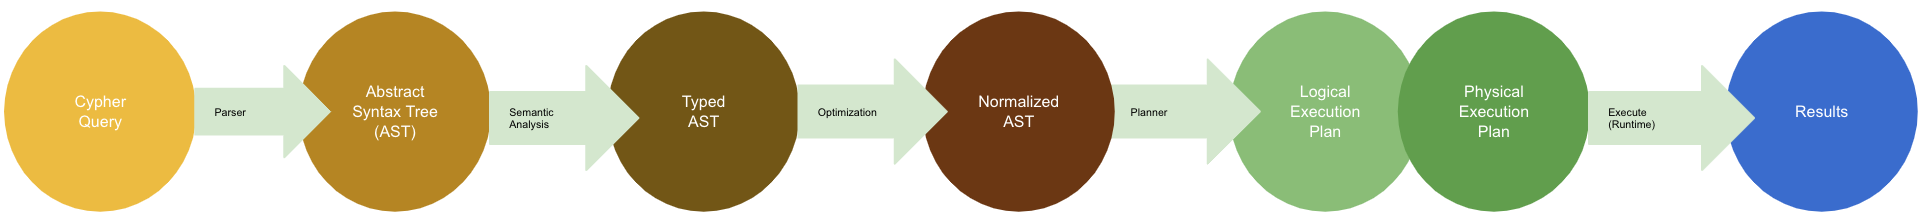
\includegraphics[width=1\textwidth]{img/low_level.png}
        \caption{Vyobrazení zpracování Cypher dotazu v Neo4j na nižší úrovni logiky\label{low_level_neo4j}.}
    \end{figure}

    \subsubsection{Popis dotazu v jazyce Cypher}
    V této podsekci bude popsán vybraný dotaz nad grafem databáze neo4j. Další vytvořené dotazu lze nalézt v přiloženém souboru \textit{queries.cypher}.

    Účelem vytvoření daného dotazu byla potřeba identifikovat všechny nehody, jejich místa a základní sídelní jednotky v městské části „Brno-střed“, ve kterých se stala dopravní nehoda, které se zúčastnila tramvaj, přičemž nehoda byla zaviněna řidičem motorového vozidla (ať již tramvaje či druhého vozidla). Cílem tohoto dotazu je určit místa v centru města, která mohou být potenciálně pro řidiče nepřehledná či složitá. Na základě získaných údajů lze provést opatření minimalizující riziko vzniku nehody, jako například přidání dopravní značky upozorňující na dávání přednosti tramvaji, úprava komunikace a jiné.

    \begin{lstlisting}[style=Cypher]
        MATCH path = (:MC {mc_val: 'Brno-střed'})<-[:NALEZI]-(:ZSJ)<-[:SPADA_DO]-(:Misto {situovani: 'na kolejích tramvaje'})<-[:LOKACI_V]-(:Nehoda)-[:Z_DUVODU]-(:Zavineni {zavineni_val: 'řidičem motorového vozidla'})
        RETURN path;
    \end{lstlisting}

    Argumentací pro potřebu takového dotazu může být nespočetný počet videí či videokanálů na internetu zachycující nehody či nebezpečné situace v Brně z pohledu řidiče tramvaje.

    Výsledkem dotazu je graf, který je vyobrazen na obrázku \ref{neo4j_query_result}. Přehled označení uzlů a relací grafu je uveden na obrázku \ref{overview}. Ten zachycuje uzel městské části „Brno-střed“ a jeho vztahy k jednotlivým místům a nehodám, které vznikly zaviněním řidiče motorového vozidla.

    \begin{figure}[ht!]
        \centering                
        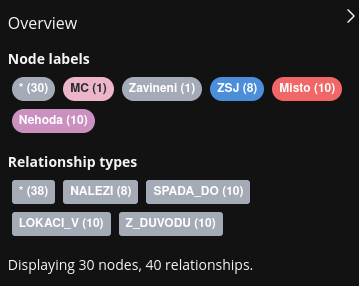
\includegraphics[width=0.45\textwidth]{img/overview.png}
        \caption{Přehled označení uzlů a relací grafu\label{overview}.}
    \end{figure}

    \begin{landscape}      
        \hfill
        \begin{figure}[ht!]
        \centering                
        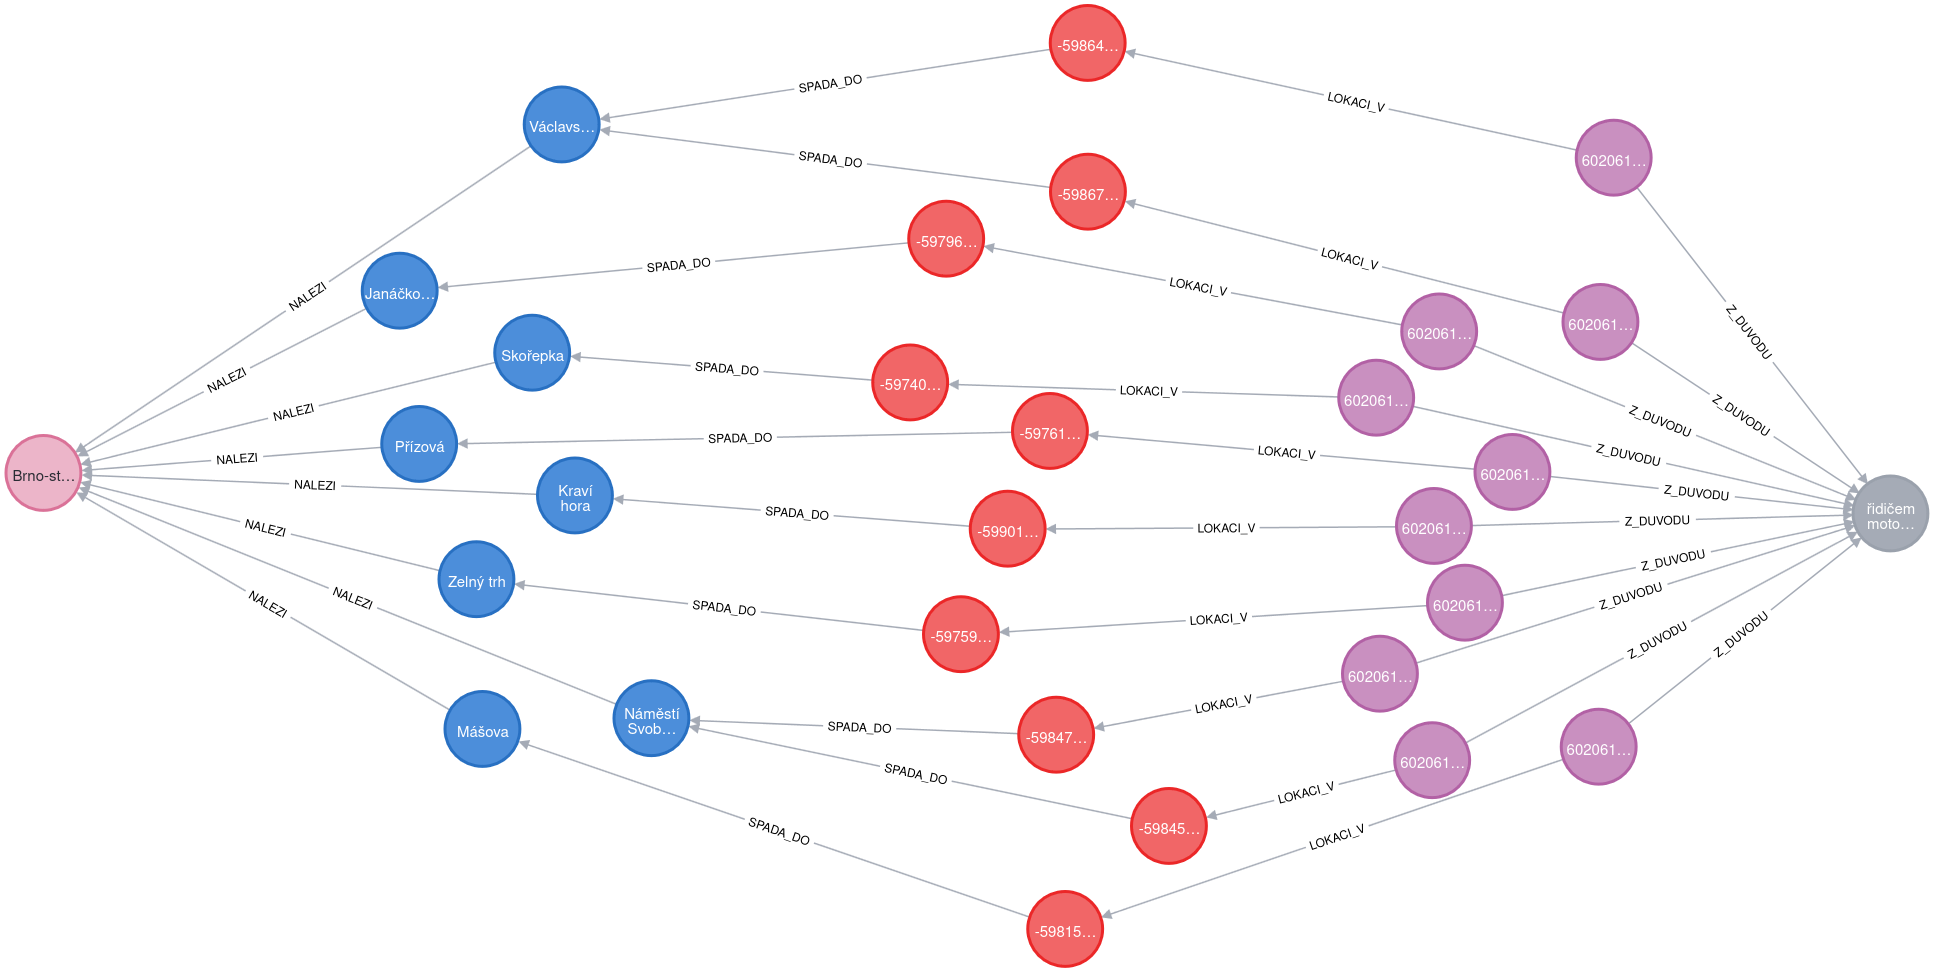
\includegraphics[width=1.5\textwidth]{img/graph.png}
        \caption{Výsledek uvedeného dotazu, který je vyobrazen ve formě grafu\label{neo4j_query_result}.}
        \end{figure}            
    \end{landscape}    

    % Štěpa
    \newpage
    \section{Databáze časových řad\,---\,InfluxDB}

    \begin{itemize}
        \item Název datové sady: Kvalita ovzduší
        \item URL: \url{https://data.gov.cz/datov%C3%A1-sada?iri=https%3A%2F%2Fdata.gov.cz%2Fzdroj%2Fdatov%C3%A9-sady%2F44992785%2F4907e5c199620d99a44c1ec388703cd5}
        \item Distribuce datové sady: CSV
    \end{itemize}

    \subsection{Rozbor charakteristik a výhod vybraného NoSQL řešení}
    InfluxDB je vhodná pro ukládání dat s časovým razítkem. Tento typ databáze umožňuje efektivní ukládání a zpracování časových dat, jako jsou časové záznamy událostí, historické údaje a sledování změn v čase. 
    
    Vybrali jsme datovou sadu, která obsahuje data z meteorologických stanic ČHMÚ\footnote{Český hydrometeorologický ústav} a Státního zdravotnického ústavu Ostrava. Jednotlivé stanice jsou rozmístěny po Brně a odesílají data v pravidelných hodinových nebo čtyřhodinových intervalech a jednou za den odešlou průměrnou hodnotu měřené veličiny. Jedná se o hodnoty ze senzorů jako jsou O3\footnote{Ozon}, PM10\footnote{Senzor pevných částic}, NO2\footnote{Oxid dusičitý}, atd.

    InfluxDB ukládá data ve formátu tzv. shluků polí. Tento přístup k ukládání dat je optimalizován pro efektivní ukládání časových řad a jejich rychlé dotazování. Data jsou ukládána ve shlucích polí, což umožňuje efektivní správu a kompresi dat. Provádí komprese například pomocí: 
    \begin{itemize}
        \item{\textbf{Kompresní algoritmy}}
        \item[]
        Tyto algoritmy pomáhají snižovat míru duplicitních nebo zbytečných dat a minimalizovat paměťové nároky.
        \item{\textbf{Sdílení hodnot}}
        \item[]
        Pokud jsou v rámci jednoho časového řádku nebo shluku polí detekovány opakující se hodnoty, InfluxDB je schopna efektivně sdílet tyto hodnoty mezi body, čímž dále snižuje potřebný prostor pro ukládání.
        \item{\textbf{Indexace a shlukování}}
        \item[]
         InfluxDB využívá indexace a shlukování k efektivnímu ukládání a rychlému vyhledávání dat. Tím se minimalizuje zátěž na disk a zvyšuje se rychlost dotazování.
    \end{itemize}

    Proto jsme zvolili tento typ databáze pro danou datovou sadu. Jedná se o data, která jsou pravidelně ukládána s časovým razítkem a jejich hodnoty jsou nejsou velmi proměnlivé, takže InfluxDB umožňuje jejich velmi efektivní uložení a pozdější dotazování.

    \subsection{Definice úložiště NoSQL databáze}

    Důležitými pojmy v InfluxDB jsou organizace, bucket, měření, značky, hodnota, časové razítko a bod. Vlastnosti v kontextu InfluxDB jsou následující:
    \begin{itemize}
        \item organizace -- Je pracovní prostor pro skupinu uživatelů. Všechny řídicí panely, úkoly, buckety a uživatelé patří do organizace.
        \item bucket -- Všechna data InfluxDB jsou uložena v bucketu. Bucket kombinuje koncept databáze a období uchování (doba trvání každého datového bodu). Každý bucket musí patřit do nějaké organizace.
        \item měření -- Měření jsou pojmenované kolekce datových bodů, které mají stejné názvy. Tyto názvy jsou obvykle spojeny s konkrétními zařízeními, senzory nebo datovými body.
        \item značky -- Značky jsou klíčové hodnoty přidělené datovým bodům v InfluxDB, které umožňují rychlé vyhledávání a filtrování dat.
        \item pole -- Pole jsou skutečná data, která jsou asociována s danými značkami. Pole mohou obsahovat různé typy dat, jako jsou čísla, text a jiné.
        \item časové razítko -- Všechna data uložená v InfluxDB mají \textunderscore time sloupec, který ukládá časová razítka.
        \item bod -- Bod obsahuje klíč řady, hodnotu pole a časové razítko.
    \end{itemize}
    Výše vypsané pojmy jsou hierarchicky vyobrazeny na následujícím obrázku:
    \begin{figure}[ht!]
        \centering
        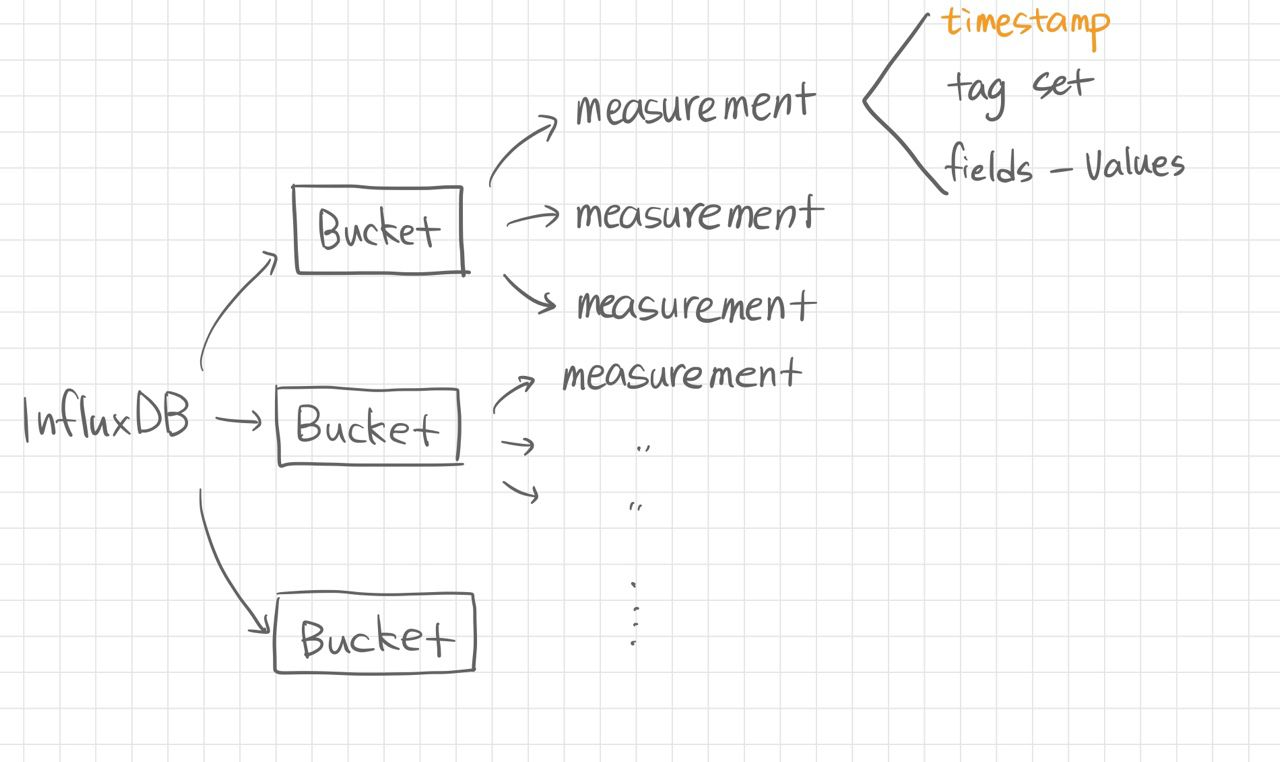
\includegraphics[width=0.8\textwidth]{img/influx.png}
        \caption{Hierarchie úložiště v InfluxDB \label{InfluxHier}}
    \end{figure}

    Pro námi zvolená data jsem zvolili následné rozdělení:
    
    \begin{table}[h!]
    \centering
    \begin{tabular}{|l|l|}
    \hline
    \textbf{Měření} & 'kvalita\_vzduchu' \\ \hline
    \textbf{Pole} &  \\ \hline
    'so2\_1h' & float \\ 
    'no2\_1h' & float \\ 
    'co\_8h' & float \\ 
    'pm10\_1h' & float \\ 
    'o3\_1h' & float \\ 
    'pm10\_24h' & float \\ 
    'pm2\_5\_1h' & float \\ \hline
    \textbf{Značky} &  \\ \hline
    'code' & string \\ 
    'name' & string \\ 
    'owner' & string \\ \hline
    \textbf{Časové razítko} & 'actualized' - time \\ \hline
    \end{tabular}
    \end{table}
    
    \subsection{Import dat}

         Pro import dat ze zvolené datové sady do NoSQL databáze InfluxDB je možné použít Influx klient CLI a nebo jednu z poskytovaných knihoven. Jelikož bude potřeba upravit počáteční data, tak jsme pro pohodlnější práci zvolili Python a knihovnu \texttt{influxdb\textunderscore client}. Postup importu dat ze zvolené datové sady vypadá následovně

         \begin{enumerate}
            \item Stažení datové sady a případné upravení struktury sady. Datovou sadu musíme pouze upravit pokud budeme chtít využít InfluxCLI.
            \item Připojení na InfluxDB server
                \begin{lstlisting}[style=Python]
            client = InfluxDBClient(url=DB_HOSTNAME, token=TOKEN, org=ORGANIZATION)
                \end{lstlisting}
                Při vyžití oficiálního kontejneru nám je poskytnuto webové rozhraní, ve kterém si vytvoříme organizaci a vygenerujeme token pro připojení.
            \item Následně si přečteme CSV soubor s daty a vytvoříme si objekt Point(bod ve výše zmíněné kapitole), který nám poskytuje již zmíněna knihovna a poté můžeme vytvořený objekt odeslat na databázový server. Zde nastavíme pouze ty hodnoty, které nám daná meteorologická stanice poskytuje.
            \begin{lstlisting}[style=Python]
            # Pole row je radek z CSV souboru
            point = Point("enviroment-control") \
                .tag('objectid', row[2] if row[2] else None) \
                .tag('code', row[3] if row[3] else None) \
                .tag('name', row[4] if row[4] else None) \
                .tag('owner', row[5] if row[5] else None) \
                .tag('lat', row[6] if row[6] else None) \
                .tag('lon', row[7] if row[7] else None) \
                .time(time=datetime.strptime(row[8], "%Y/%m/%d %H:%M:%S+00"))
            
                # Nastavujeme pouze pokud hodnota je poskytnuta
                if row[9]:
                    point.field('so2_1h', float(row[9]))
                if row[10]:
                    point.field('no2_1h', float(row[10]))
                if row[11]:
                    point.field('co_8h', float(row[11]))
                if row[12]:
                    point.field('pm10_1h', float(row[12]))
                if row[13]:
                    point.field('o3_1h', float(row[13]))
                if row[14]:
                    point.field('pm10_24h', float(row[14]))
                if row[15]:
                    point.field('pm2_5_1h', float(row[15])) 
                \end{lstlisting}
            \item Po dokončení importu je vhodné ukončit navázané spojení se serverem.
        \end{enumerate}

            Celý tento postup je zkompletován v přiloženém Python skriptu nesoucí název \texttt{influx.py} a je možné ho spustit pomocí 
    následujícího příkazu příkazu:
    \begin{lstlisting}[style=Python, language=Python, framesep=10pt]
        $ python3 influx.py -f kvalita_ovzdu.csv
    \end{lstlisting}

        \subsubsection{Vkládání/aktualizování dat do existujícího měření}
        Pro vkládání/aktualizování dat v InfluxDB můžeme použít stejný Python skript, který je zmíněný výše. Kolize databáze řeší tak, že při zápisu bodu se stejným měřením, sadou značek a časovým razítkem jako existující bod dojde k přepsání původního bodu novými hodnotami. Pokud je kombinace časového razítka, měření a značek unikátní, InfluxDB bod vloží jako nový záznam. Samotní vývojáři ale časté aktualizování hodnot nedoporučují, protože InfluxDB není pro to velmi optimalizovaný, kvůli již zmíněným kompresím uložených dat.
    
    \subsection{Dotaz v jazyce databázového produktu}
    
        Pro správné pochopení, jak InfluxDB zpracovává dotaz, je možné postup rozdělit do několika klíčových kroků, kde jednotlivé kroky postupu jsou popsány níže

        \begin{enumerate}
            \item Příjem dotazu -- Dotaz je přijat hlavním uzlem nebo koordinátorem, který slouží jako vstupní bod pro klienty.
            \item Určení umístění dat -- Koordinátor identifikuje, na kterých uzlech jsou uložena požadovaná data. V distribuovaném systému mohou být data replikována na více uzlech pro zvýšení dostupnosti a odolnosti.
            \item Paralelní zpracování -- Dotaz je rozeslán na všechny relevantní uzly. Každý uzel zpracuje část dotazu na svých lokálních datech. To umožňuje paralelní zpracování, což může výrazně zrychlit celkový čas zpracování, zejména pro velké datové sady.
            \item Agregace výsledků -- Po zpracování části dotazu na každém uzlu jsou výsledky odeslány zpět koordinátoru. Koordinátor pak agreguje výsledky z jednotlivých uzlů do konečné odpovědi, která je odeslána klientovi.
        \end{enumerate}
    
        Pro dotazování nad InfluxDB využijeme jejich CLI klienta. Po nainstalování se musíme připojit k serveru pomocí následujícího příkazu.
        \begin{lstlisting}[style=Python]
            influx config create --config-name <config-name> \
              --host-url https://us-west-2-1.aws.cloud2.influxdata.com \
              --org <your-org> \
              --token <your-auth-token> \
              --active
        \end{lstlisting}
        Ověřit správné připojení na databázoví server můžeme pomocí příkazu \texttt{influx server-config}, který nám při správném nastavení vrátí informace o InfluxDB serveru. InfluxDB podporuje několik způsobů dotazování a interakce s daty:

        \begin{itemize}
            \item \textbf{InfluxQL a Flux}: SQL-podobné dotazovací jazyky pro práci s daty. InfluxQL je podporován v InfluxDB 1.x, zatímco Flux je k dispozici v InfluxDB 2.x a novějších.
            \item \textbf{HTTP API}: Umožňuje dotazování a správu databáze prostřednictvím HTTP požadavků.
            \item \textbf{Klientské knihovny}: Pro různé programovací jazyky, např. Python, Java, Go, JavaScript.
            \item \textbf{Grafické rozhraní}: Chronograf pro InfluxDB a Grafana pro vizualizaci dat.
        \end{itemize}
        \begin{lstlisting}[style=Python]
         $ influx query -r 'from(bucket: "vut")
          |> range(start: 2023-08-01T00:00:00Z, stop: 2023-08-31T23:59:59Z)
          |> filter(fn: (r) => r["_measurement"] == "air-control")
          |> filter(fn: (r) => r["name"] == "Brno - Detska nemocnice")
          |> filter(fn: (r) => r["_field"] == "pm10_1h")
          |> aggregateWindow(every: 6h, fn: mean, createEmpty: false)
          |> yield(name: "mean")'
        \end{lstlisting}
        Ve výpisu vidíme příkaz v jazyce Flux pro InfluxDB. Dotazujeme se na data z bucketu \texttt{vut} pro měření \texttt{air-control} na stanici \texttt{Brno - Dětská nemocnice}. Konkrétně se zaměřuje na hodnoty pole \texttt{pm10\textunderscore1h}, které reprezentují hodinové koncentrace částic PM10. Dotaz vybírá data za srpna 2023 a agreguje je do šestihodinových intervalů, přičemž vypočítává průměrnou hodnotu v každém z nich. Příkaz můžeme provést i poskytnutém webovém rozhraní, kde si výsledek můžeme nechat zobrazit v grafu, který vidíme na následujícím obrázku.
        \begin{figure}[ht!]
        \centering
        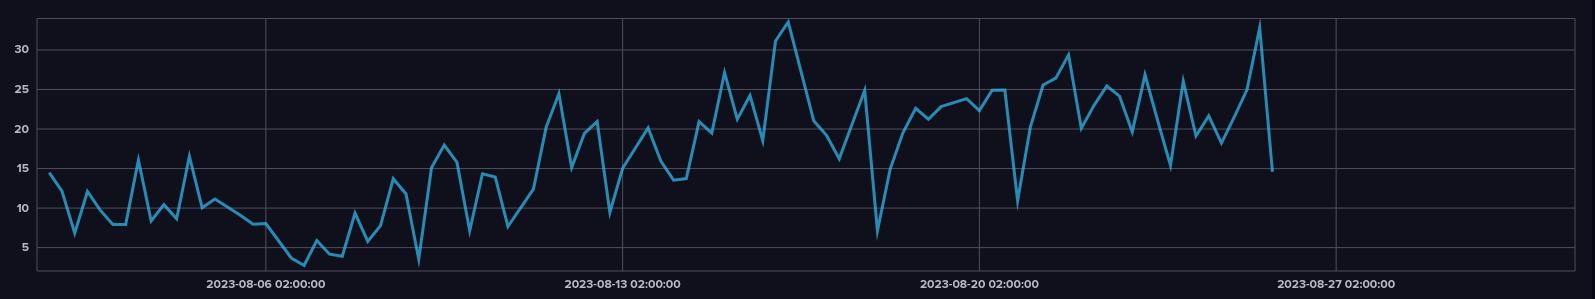
\includegraphics[width=1\textwidth]{img/inflexGraf.png}
        \caption{Graf z výsledků dotazu \label{InfluxGraf}}
    \end{figure}

    
    
\end{document}